\section{Traitement et visualisation des données}
\subsection{Stitching}
Une fois l'acquisition terminée, le fichier de données se trouve dans le répertoire déterminé à la section \ref{start}. Afin de 'stitcher' (assembler les tuiles) les données, il faut ouvrir l'application MATLAB se trouvant dans la barre de tâches.


\begin{figure}[H]
    \centering
    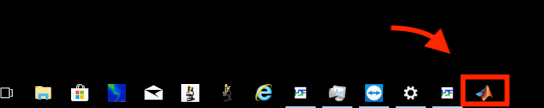
\includegraphics[scale = 0.7]{taskbar.png}
    \caption{Ouvrir MATLAB}
    \label{fig:task_bar}
\end{figure}

Une fois MATLAB ouvert, assurez-vous que vous êtes bien dans le répertoire 'LightsheetUtilities', comme à la figure~\ref{fig:repertpoire}.

\begin{figure}[H]
    \centering
    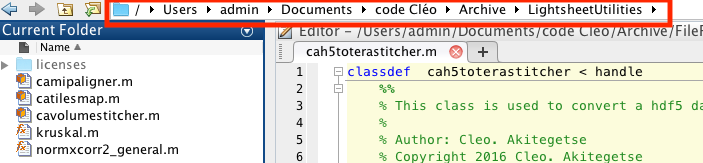
\includegraphics[scale = 0.7]{repertoire.png}
    \caption{Répertoire LightsheetsUtilities}
    \label{fig:repertpoire}
\end{figure}

\begin{figure}[H]
    \centering
    \subfloat{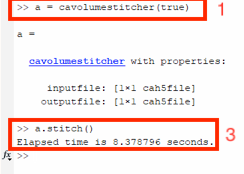
\includegraphics[width=6cm]{1-3.png} }%
    \qquad
    \subfloat{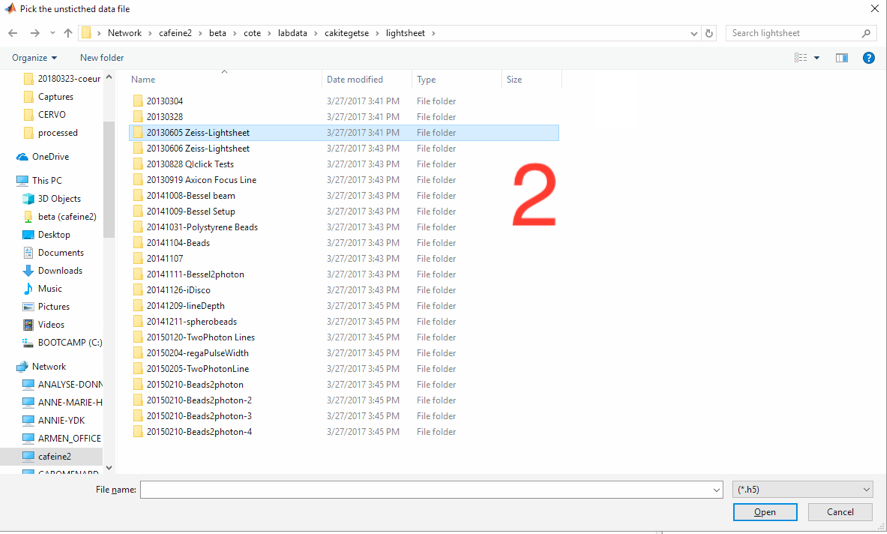
\includegraphics[width=9cm]{2.png} }%
    \caption{Les 3 étapes pour 'stitcher' les données}%
    \label{fig:cmd}%
\end{figure}

Exécutez la commande suivante (1) dans la fenêtre de commande de MATLAB.
$$>>a = cavolumestitcher(true) $$

Comme illustré à la figure \ref{fig:cmd}, une fenêtre apparaîtra afin que l'utilisateur puisse sélectionner  les données qu'il aimerait 'stitcher'. Une fois le fichier sélectionné, les informations sur celui s'afficheront dans la fenêtre de commande. Afin de terminer le traitement des données, l'utilisateur doit entrez la commande suivante (3):
$$>>a.stitch()$$

Cette opération peut être longue dépendamment de la grosseur du fichier. Une barre de progression sera affichée à l'écran. Le fichier créer par cette dernière étape sera enregistré dans le même répertoire que le fichier d'origine contenant les données non traitées.

\subsection{Visualisation 3D}
Afin de visualiser les données, ouvrez l'application 'Vaa3D' se trouvant dans la barre de tâches.

\begin{center}\textcolor{red}{***Attention! Assurez vous qu'aucun fichier temporaire du genre 'vmap.bin' se trouve dans le répertoire dans lequel se trouve le fichier que vous désirez ouvrir. En présence d'un tel fichier, supprimez-le. ***}\end{center}


\begin{figure}[H]
    \centering
    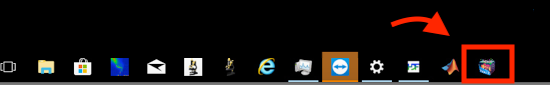
\includegraphics[scale = 0.7]{taskbar2.png}
    \caption{Ouvrir Vaa3D}
    \label{fig:vaad}
\end{figure}

Une fois l'application en ouverte, lancez le plugin TeraFly en suivant les étapes de la figure~\ref{fig:big}.

\begin{figure}[H]
    \centering
    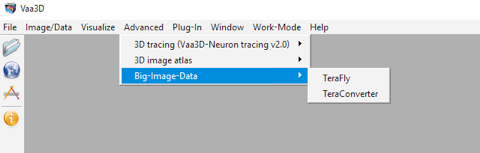
\includegraphics[scale = 0.7]{big.png}
    \caption{ Ouverture du plugin TeraFly}
    \label{fig:big}
\end{figure}

À partir de TeraFly, vous pouvez ouvrir le fichier que vous venez de traiter en suivant les étapes de la figure~\ref{fig:tera}.

\begin{figure}[H]
    \centering
    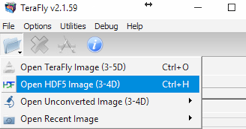
\includegraphics[scale = 1]{tera.png}
    \caption{Ouverture de fichier via TeraFly}
    \label{fig:tera}
\end{figure}

Les données seront visibles sous forme d'un volume. Il est possible de naviguer dans le volume et d'agrandir certaine section.